
	Une athlète a réalisé un triathlon d’une longueur totale de 12,9 kilomètres. Les trois épreuves se déroulent dans l’ordre suivant :
	
	\begin{center}
		\begin{tabularx}{14 cm}{|*{3}{>{\centering \arraybackslash}X|}} \hline
		Épreuve \tikz[baseline=(x.base)]{\draw (0,0) circle (8pt) node (x) {1};}\rule{0pt}{14pt} :     & Épreuve \tikz[baseline=(x.base)]{\draw (0,0) circle (8pt) node (x) {2};} :     & Épreuve \tikz[baseline=(x.base)]{\draw (0,0) circle (8pt) node (x) {3};} : \\
		Natation          & Cyclisme          & Course à pied. \\
		Distance = 400 m  &                   & Distance = 2,5 km\\ \hline
		\end{tabularx}
	\end{center}

	Entre deux épreuves, l’athlète doit effectuer sur place un changement d'équipement.
	
	Le graphique ci-dessous représente la distance parcourue (exprimée en kilomètre) par l’athlète, en fonction du temps de parcours (exprimé en minute) de l’athlète pendant son triathlon.
	
	\begin{center}
		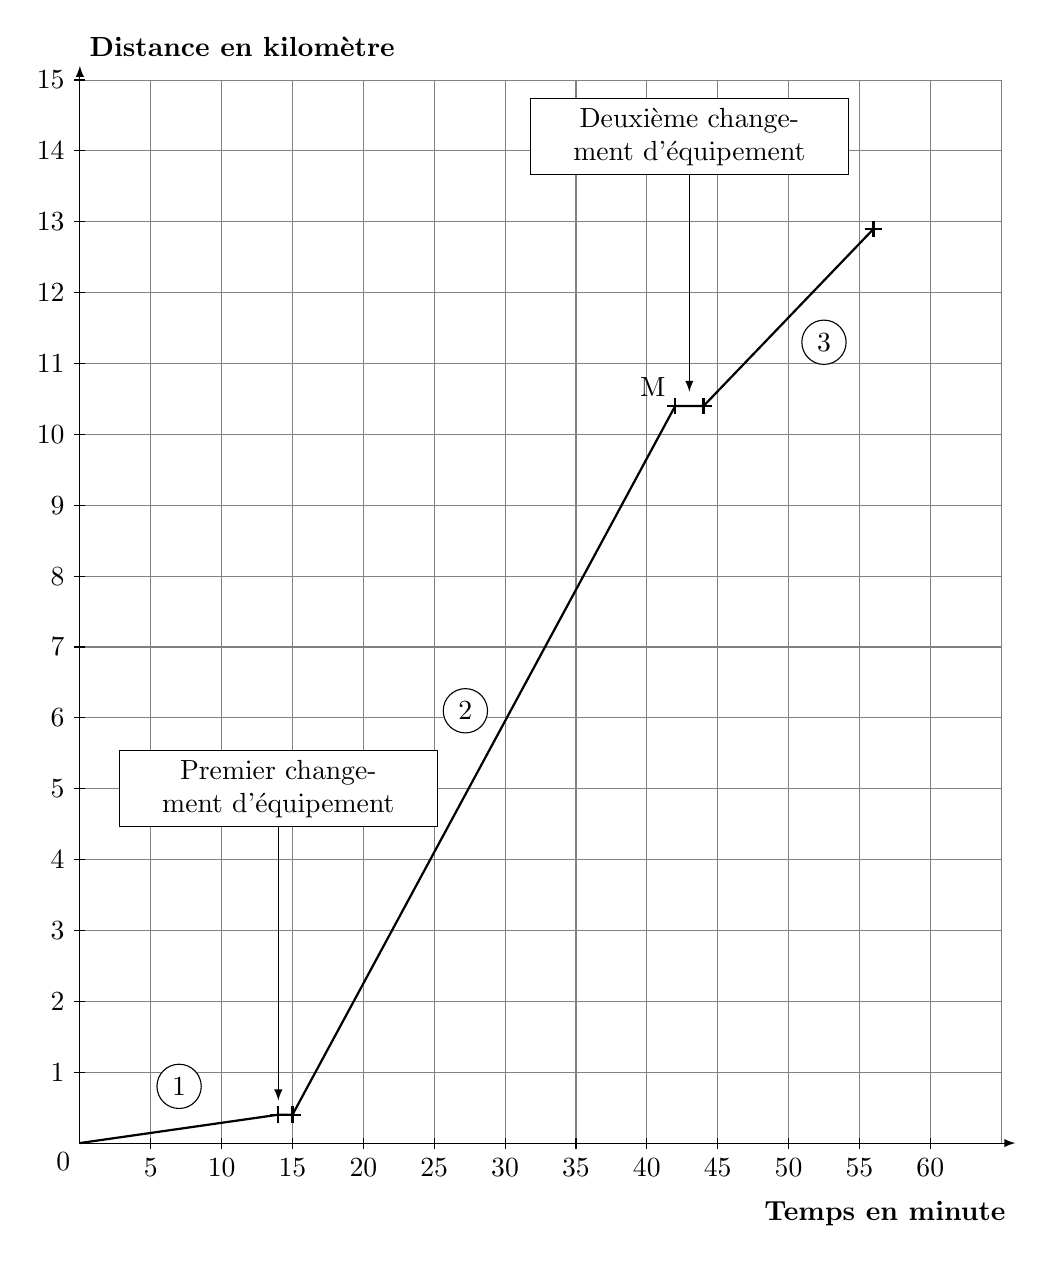
\begin{tikzpicture}[x=1.8mm,y=9mm,> = latex]
			\draw [gray,xstep=5,ystep=1] (0,0) grid (65,15);
			\draw[<->] (0,15.2) node [above right] {\textbf{Distance en kilomètre}}--(0,0)--(66,0) node[shift={(0,-1)}, left] {\textbf{Temps en minute}};
			\foreach \x in {5,10,...,60}{
				\draw (\x,2pt)--(\x,-2pt) node [below] {\x};}
				%%%%%%%%
           \foreach \y in {1,2,...,15}{
                \draw (2pt,\y)--(-2pt,\y) node [left] {\y};}
            \node at (0,0) [below left] {0};
	
				%%%%%%%%
			\draw[line width=0.8pt] (0,0)--(14,0.4)--(15,0.4)--(42,10.4)--(44,10.4)--(56,12.9);
			\foreach \c in {(14,0.4),(15,0.4),(42,10.4),(44,10.4),(56,12.9)}
				\draw[shift=\c,line width=0.8pt] (-3pt,0)--(3pt,0) (0,3pt)--(0,-3pt);
			\draw[fill = white] (7,.8) circle (8pt) node (x) {1};
			\draw[fill = white] (27.2,6.1) circle (8pt) node (y) {2};
			\draw[fill = white] (52.5,11.3) circle (8pt) node (z) {3};
			\draw (42,10.4) node[above left] {M};
			\draw[<-](14,0.6)--(14,5) node[text width=38 mm, align = center, fill=white, draw] {Premier changement d'équipement};
			\draw[<-](43,10.6)--(43,14.2) node[text width=38 mm, align = center, fill=white, draw] {Deuxième changement d'équipement};
		\end{tikzpicture}
	\end{center}	

Le point M a pour abscisse 42 et pour ordonnée 10,4.
	
À l’aide du tableau ci-dessus ou par lecture du graphique ci-dessus avec la précision qu’il permet, répondre aux questions suivantes, en justifiant la démarche.

\medskip
	
	\begin{enumerate}
		\item Au bout de combien de temps l’athlète s’est-elle arrêtée pour effectuer son premier changement d'équipement ?
		
		\item Quelle est la longueur, exprimée en kilomètre, du parcours de l'épreuve de cyclisme ?
		
		\item En combien de temps l’athlète a-t-elle effectué l'épreuve de course à pied ?
		
		\item Parmi les trois épreuves, pendant laquelle l’athlète a été la moins rapide ?
		
		\item On considère que les changements d'équipement entre les épreuves font partie du triathlon.
		
		La vitesse moyenne de l’athlète sur l’ensemble du triathlon est-elle supérieure à 14 km/h ?
	\end{enumerate}
	
	
